\chapter{Anteproyecto}

\section{Descripción y Alcance del proyecto}
\subsection{Antecedentes}
%¿Quién solicita el proyecto? ¿Cuál es el departamento, oficina o grupo que requiere el proyecto y a qué se dedican? - Respalde con citas bibliográficas.

%¿Cuál es la necesidad que el grupo tiene por la que requieren desarrollar este proyecto? ¿Cómo el proyecto va a solventar esa necesidad? ¿Cuál va a ser el impacto del proyecto? ¿Qué beneficios traerá el proyecto y para quién? ¿Hay un sector de la población cuya calidad de vida mejorará gracias a la implementación de este proyecto? ¿Cuál es ese grupo?

Este proyecto surge como respuesta a una necesidad directa expresada por el cliente Rodolfo Mora, quien en la actualidad usa distintos lectores de PDF y manifiesta una insatisfacción con estas herramientas debido a sus interfaces sobrecargadas de utilidades, barras de herramientas y menús poco intuitivos. Además, también menciona experiencias negativas con lectores alternativos, que son más livianos, pero tienen algunos problemas de estabilidad, entre otras cosas.

Otro problema mencionado corresponde a la firma electrónica de documentos. El cliente utiliza actualmente un firmador que fue desarrollado en Java y presenta una limitación importante: esta firma utiliza siempre el tamaño original de la imagen sin posibilidad de re-posicionar o ajustarla en el espacio disponible en el documento, provocando superposiciones con el texto u otros elementos.

Tomando en cuenta lo anterior, dentro de las funciones específicas mencionadas por el cliente está el manejo de archivos de presentaciones PPT que fueron transformadas a PDF, por lo que la aplicación debe contar con un modo presentación que le permita manipularlas para visualizarlas correctamente dispositiva por diapositiva. También debe permitir la edición de documentos de carácter legal que requieren ser firmados con validez legal utilizando el sistema de firmas digitales GAUDI del Banco Central de Costa Rica, pudiendo posteriormente verificar dicha firma en el propio sistema GAUDI. Y finalmente, se debe tomar en cuenta la posibilidad de editar documentos, ya sea con ediciones visuales o de contenido al mezclar o compaginar PDF's.

Como referencia de estilo visual el cliente resaltó la interfaz que utiliza un lector desarrollado por Augmented Text Company (\url{https://www.augmentedtext.info/reader}), que corresponde a un visor sin barra de título, sin bordes intrusivos y con un estilo minimalista blanco sobre blanco agradable a la vista.

\subsubsection{Beneficiario}
El beneficiario directo del proyecto es el cliente Rodolfo Mora, quien en su labor académica maneja de forma constante documentos en formato PDF (lecturas, presentaciones exportadas y documentos legales que requieren firma), y que actualmente no cuenta con una herramienta
que combine una interfaz minimalista con las funcionalidades específicas que necesita.

\subsubsection{Importancia}
La importancia del proyecto radica en ofrecer una alternativa amigable a las aplicaciones de lectura y edición de PDF existentes en el mercado que, según lo expresado por el cliente, priorizan la cantidad de funcionalidades visibles por encima de la experiencia de lectura sobrecargando la interfaz y dificultando la concentración en el contenido. Adicionalmente resuelve una necesidad concreta del cliente respecto a la firma electrónica de documentos, al integrar un mecanismo reposicionable y compatible con el sistema oficial de GAUDI del BCCR, de forma que se evitarían las limitaciones de las herramientas que utiliza actualmente.

\subsubsection{Grupos o comunidades beneficiadas}

El principal beneficiado es el cliente. Sin embargo, dado que se contempla como un proyecto de software libre, cualquier usuario de Windows (y eventualmente Linux) que busque un lector y editor de PDF minimalista, con soporte a anotaciones, firma electrónica y manejo de formatos adicionales (EPUB, DVI Y Markdown), podrá beneficiarse de la herramienta desarrollada.

\subsubsection{Necesidades solventadas}

\begin{enumerate}
	\item Interfaces sobrecargadas y poco intuitivas de los lectores de PDF actualmente disponibles (Adobe Acrobat, Foxit, entre otros), que dificultan una experiencia de lectura centrada en el contenido.
	\item Ausencia de una solución de firma electrónica agil, compatible con el sistema GAUDI del Banco Central de Costa Rica, que permita ajustar el tamaño y la posición de la firma gráfica sobre el documento, a diferencia de las herramientas actuales utilizadas por el cliente.
	\item Falta de un medio para anotar, resaltar y comentar documentos PDF de forma sencilla y, en la medida de lo posible, interoperable con otros lectores del mercado.
	\item Necesidad de trabajar con múltiples formatos de documento (PDF, EPUB, DVI y Markdown) desde una única herramienta, incluyendo la conversión de carpetas completas de archivos Markdown en un único documento PDF.
\end{enumerate}

\subsection{Objetivos}

%
% Los objetivos del proyecto deben englobar el alcance total. Todo objetivo debe estar redactado respetando la siguiente estructura:

% Verbo infinitivo: Representa una acción que el equipo de desarrollo ejecutará durante el proyecto. Debe ser una acción concreta y relevante para completar el proyecto

% Objeto: Indica el objeto sobre el cual se aplicará la acción. Típicamente representa el producto esperado de la acción

% Modo: Indica parámetros por los cuales se medirá la calidad y completitud del resultado. 

% Ejemplo: Desarrollar un sistema de facturación electrónica que provea una interfaz amigable para el usuario y cumpla con los estándares impuestos por el Ministerio de Hacienda de Costa Rica. 

% Sólo puede existir un verbo infinitivo en el objetivo
% Debe ser posible medir el nivel de cumplimiento del objetivo, es decir, debe ser posible decir en cualquier momento del proyecto, cual porcentaje del objetivo se ha cumplido.

\begin{itemize}
    \item \textbf{Objetivo General}
    \begin{itemize}
        \item Desarrollar una aplicación de escritorio para Windows que permita visualizar, anotar, firmar electrónicamente y combinar documentos PDF, así como abrir y exportar documentos en otros formatos compatibles, mediante el uso de tecnologías como Electron, HTML, CSS, JavaScript, y PDF.js.
    \end{itemize}
    \item \textbf{Objetivos Específicos}
    \begin{itemize}
        \item Desarrollar un módulo de visualización y gestión de documentos PDF que permita abrir, renderizar, mezclar y presentar documentos.
        \item Implementar un módulo de anotación de documentos PDF que permita resaltar texto y agregar comentarios.
        \item Implementar un módulo de firma electrónica de documentos PDF que permita incorporar firmas digitales y verificar su validez mediante mecanismos de validación establecidos por el sistema GAUDI (Gestor de Autenticación Digital) del Banco Central de Costa Rica.
        \item Desarrollar un módulo de gestión de documentos que permita editar documentos PDF e importar y exportar documentos en formatos PDF, EPUB, DVI, y Markdown.
        
    \end{itemize}
\end{itemize}

\subsection{Interesados}
% Liste los diferentes involucrados en este proyecto, incluya en una figura un organigrama en el cual se ilustre la relación entre todos los participantes e interesados con los miembros del equipo de trabajo.

\begin{table}[H]
    \centering
    \begin{tabular}{l|l|l}
        \textbf{Nombre del involucrado} & \textbf{Rol} & \textbf{Contacto}\\
        \hline \hline
        Rodolfo Mora Zamora & Cliente & rodmora@itcr.ac.cr\\ 
        Rodolfo Mora Zamora & Profesor & rodmora@itcr.ac.cr\\ 
        Samuel Zúñiga Vega & Desarrollador & sazuniga@estudiantec.cr\\
        Fabián Araya Ortega & Desarrollador & fabianarayaortega@estudiantec.cr\\
        Andrés Feng Wu & Desarrollador & anfeng@estudiantec.cr\\
        Rubén Hurtado Granados & Desarrollador & rhurtado@estudiantec.cr\\ 
        Víctor Mejías Salas & Desarrollador & vmejias@estudiantec.cr\\ 
        Xotchil Rojas Fernández& Desarrollador & xorojas@estudiantec.cr\\ 
        \hline
    \end{tabular}
    \caption{Involucrados del proyecto}
    \label{tab:my_label}
\end{table}

% Organigrama
\begin{figure}[H]
  \centering
    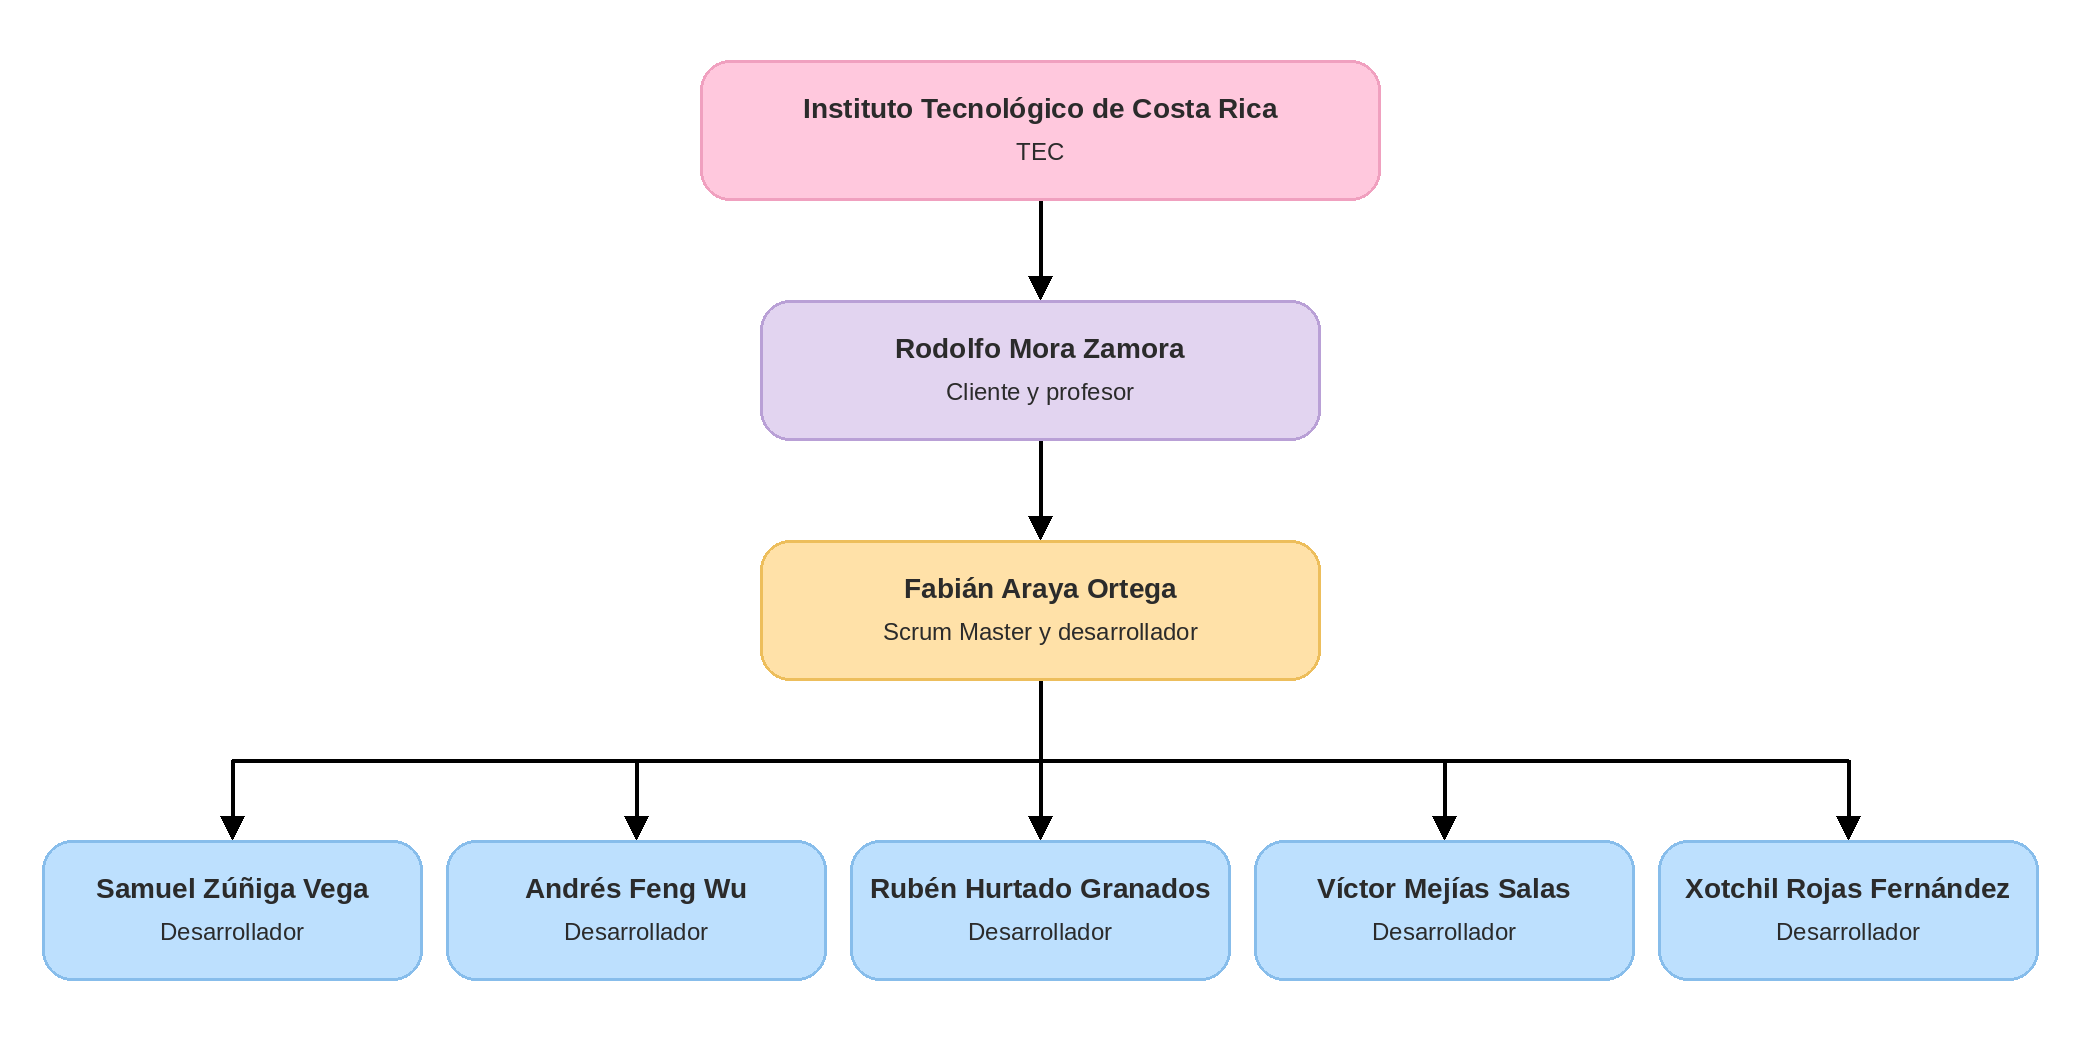
\includegraphics[height= 8cm, width=15cm]{project/images/organigrama.png}
  \caption{\textbf{Relación entre los participantes e interesados con los miembros del equipo de trabajo}}
\end{figure}

\subsection{Estructura de Desglose de Trabajo}

%Divida su proyecto en cuatro Productos Mínimos Viables (MVP por sus siglas en inglés),  cada MVP debe descomponerlo en entregables que deberá presentar a su cliente al final de cada iteración. Describa cada MVP en esta sección, indicando en cuáles subproductos se divide.

%Diagrame sus entregables en una Estructura de Desglose de Trabajo (EDT) que le facilite llevar un registro de cuáles se deben cumplir en cada etapa del proyecto. Utilice esta guía para orientarse en cómo desarrollar su EDT: https://formulaproyectosurbanospmipe.wordpress.com/2012/05/09/tema-n-5-la-estructura-de-desglose-del-trabajo-edt-segun-la-guia-del-pmbok-30-04-2012-sesion-10-segunda-parte/.

Como se mencionó anteriormente, se creará una aplicación minimalista que permita la lectura y edición de archivos PDF, así como implementación de la firma digital con GAUDI y distintos formatos. Para lograrlo, el proyecto se dividirá en 3 etapas que producirán un MVP cada una:

\begin{enumerate}
    \item Primer prototipo de aplicación: Contendrá la aplicación de escritorio con la interfaz minimalista base, esto incluye el menú lateral, el menú contextual y las funciones de: buscar, seleccionar y copiar texto, guardar un archivo pdf, desplazar las páginas, hacer zoom al documento y edición básica como reordenar páginas o eliminarlas. Además, permitirá visualizar archivos PDF, así como mezclar y compaginar varios PDFs en un solo archivo. Incluirá también el modo presentación y la visualización del outline (estructura) del documento. 
    \item Aplicación con firma digital y anotaciones: Este entregable contará con todas las características del prototipo, con adición de la integración del uso de la firma digital electrónica GAUDI del Banco Central de Costa Rica. Además, extenderá la función de edición al permitir resaltar (highlight) texto dentro del documento, agregar comentarios y realizar firmas gráficas sobre el PDF.
    \item Aplicación con soporte multi-formato: Este será el último entregable y contendrá todas las características respecto a la gestión de formatos, como abrir archivos EPUB, DVI y Markdown, así como exportar entre estos formatos y PDF. Se incluirá la funcionalidad para convertir una carpeta completa de archivos Markdown en un único documento PDF. Finalmente se realizará un empaquetado general de la aplicación para su distribución en Windows (y Linux, en caso de completarse el soporte contemplado).
\end{enumerate}

De ser posible, y habiendo cumplido con todos los requerimientos anteriores, se agrega un cuarto entregable que consiste en la aplicación con soporte para Linux.

% EDT
\begin{figure}[H]
  \centering
    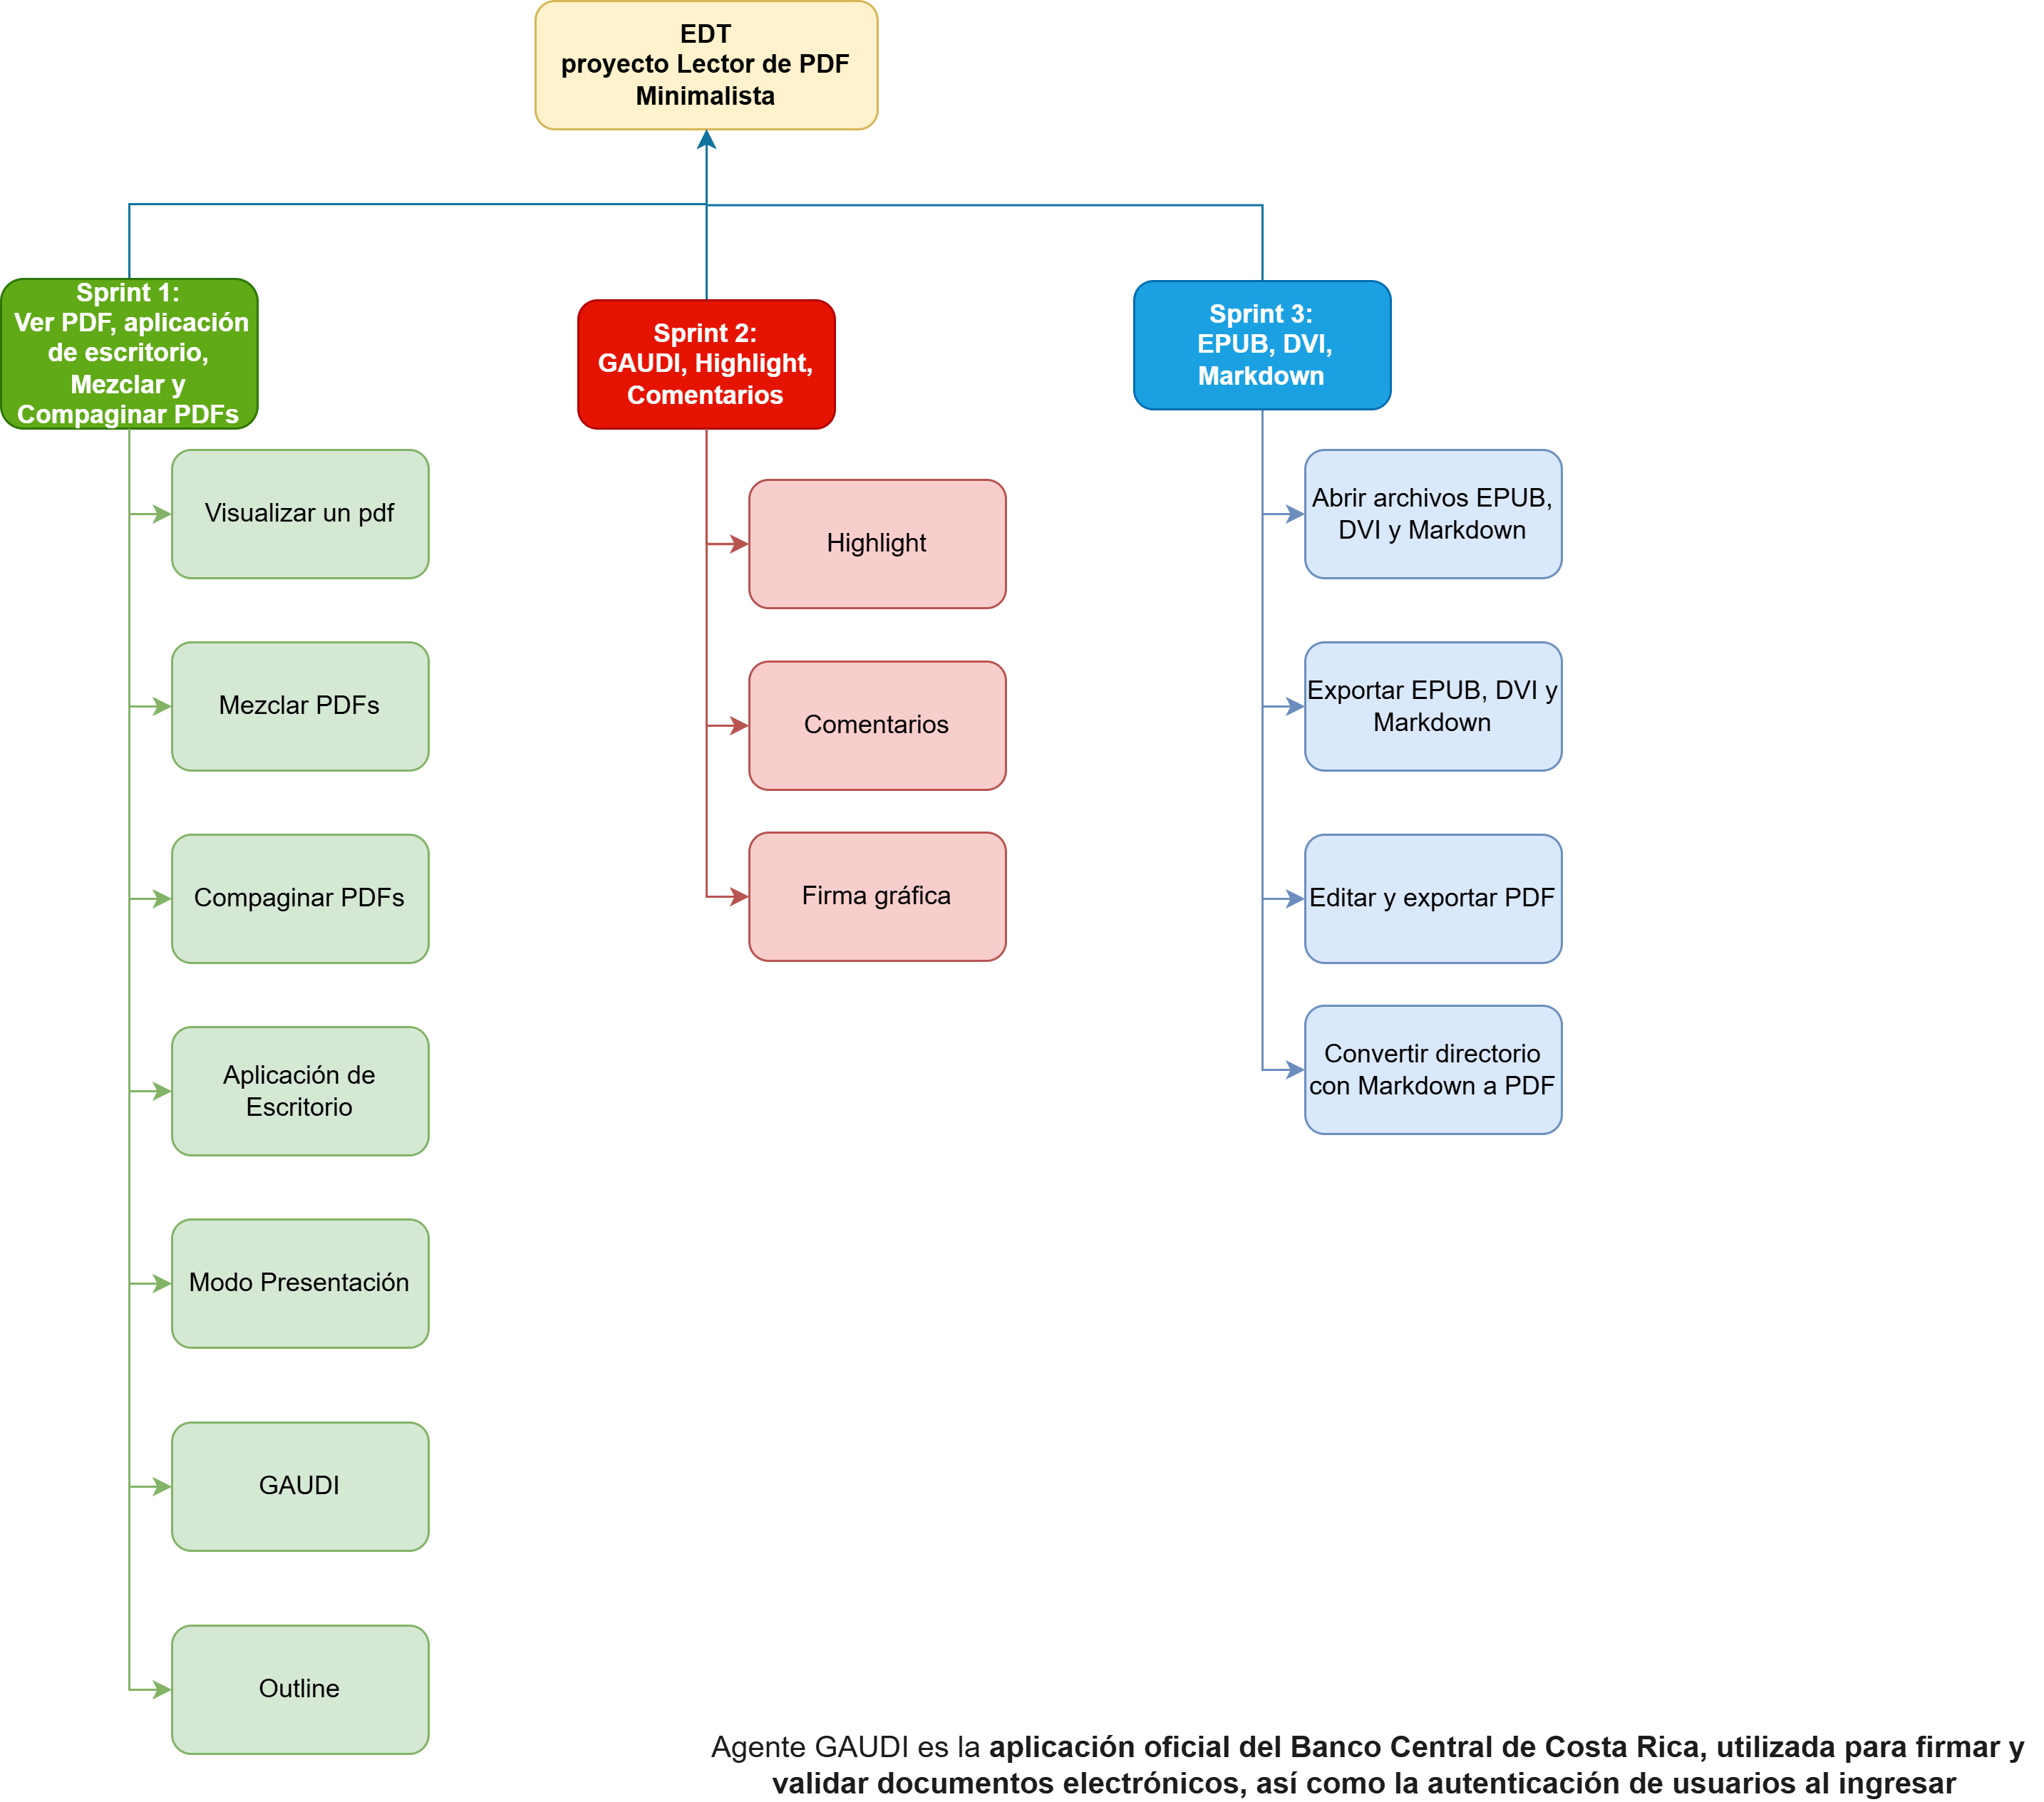
\includegraphics[height= 15cm, width=15cm]{project/images/EDT.png}
  \caption{\textbf{EDT del Lector de PDF Minimalista}}
\end{figure}
